\section{Conceitos elementares de Forth}

\begin{frame}[fragile]{Palavras}

    \begin{itemize}
        \item Forth organiza seus códigos por meio de comandos nomeados, que abstram tarefas
            ou ações correlacionadas por meio de um nome comum

        \item Estes comandos nomeados seriam os equivalentes a funções em outras linguagem

        \item A sintaxe para a criação de um novo comando é

            \inputsyntax{forth}{codes/word.fs}
        
        ou seja, inicia com dois-pontos, segue com o nome e continua com a definição, que termina
        com ponto-e-vírgula

        \item Comandos definidos dessa forma são denominados \textbf{palavras} (\textit{words})

        \item O padrão ANS da linguagem disponibiliza um conjunto grande (mais de 300) palavras
            pré-definidas, que podem ser usadas para definir novas palavras

        \item A habilidade de definir palavras por meio de palavras já definidas é denominada
            \textbf{extensibilidade}
    \end{itemize}

\end{frame}


\begin{frame}[fragile]{Modo interativo}

    \begin{itemize}
        \item No modo interativo do Forth (REPL), o interpretador responde aos comandos executados
            de forma bem sucedida com a palavra ``\code{forth}{ok}''

        \item Por exemplo, entre no modo interativo e digite a tecla \texttt{ENTER}: Forth responderá 
            ``\code{forth}{ok}'', movendo o cursor para a próxima linha

        \item Para inserir um ou mais números na pilha, basta inseri-los, na ordem desejada e 
            separados por um espaço em branco, e digitar \texttt{ENTER}

        \item Para visualizar o estado atual da pilha, use a palavra \code{forth}{.s}, a qual não
            tem parâmetros

            \inputcode{forth}{codes/stack.fs}
    \end{itemize}
\end{frame}

\begin{frame}[fragile]{Palavras para a manipulação do terminal}

    \begin{itemize}
        \item Quando uma palavra recebe um ou mais argumentos, eles são extraídos da pilha, 
            do último para o primeiro

        \item Por exemplo, a palavra \code{forth}{spaces} recebe um argumento $n$ e imprime $n$
            espaços no terminal

            \inputcode{forth}{codes/spaces.fs}

        \vspace{0.1in}

        \item A palavra \code{forth}{emit} recebe um inteiro $n$ imprime no terminal o caractere
            cujo código ASCII é $n$:

            \inputcode{forth}{codes/emit.fs}

    \end{itemize}

\end{frame}

\begin{frame}[fragile]{Palavras para a manipulação do terminal}

    \begin{itemize}
        \item O código abaixo define uma nova palavra, chamada \code{forth}{STAR}, que imprime um 
            asterisco no terminal:

            \inputcode{forth}{codes/star.fs}

        \vspace{0.1in}

        \item Também é possível definir uma nova palavra, chamada \code{forth}{STARS}, que recebe
            um argumento $n$ e imprime $n$ asteriscos consecutivos:

            \inputcode{forth}{codes/stars.fs}

    \end{itemize}

\end{frame}

\begin{frame}[fragile]{O dicionário}

    \begin{itemize}
        \item Todas as palavras definidas em Forth, seja em biblioteca padrão, seja pelo usuário, são
            armazenadas no ``dicionário''

        \item Quando uma nova palavra é definida, Forth compila a palavra e a insere em seu dicionário

        \item Por exemplo, a linha abaixo é uma definição alternativa para a palavra \code{forth}{STAR}:
            (\code{forth}{[CHAR]} traduz o caractere para seu código ASCII):

            \inputsyntax{forth}{codes/star2.fs}

        \item Quando um comando é inserido no terminal, 
            será ativada a palavra \code{forth}{INTERPRET}, que fará a leitura da entrada em busca
            de uma string (sequência de caracteres separada por espaços em branco)
    \end{itemize}

\end{frame}

\begin{frame}[fragile]{O dicionário}

    \begin{itemize}
        \item Se a palavra encontrada consta no dicionário,
            será ativada a palavra \code{forth}{EXECUTE}, que executa a definição da palavra e 
            finaliza com a mensagem ``\code{forth}{ok}''

        \item Se a palavra não consta no dicionário, então Forth tentará interpretar a string
            como um número: caso ele tenha sucesso na conversão, o número lido será 
            inserido na pilha

        \item Se a palavra lida não é um número, Forth sinaliza um erro, indicando que a palavra
            não foi definida

        \item Os nomes das novas palavras devem ser compostos por, no máximo, 31 caracteres imprimíveis

        \item Por exemplo, a palavra \code{forth}{."}, que imprime no terminal a string que se segue,
            delimitada por aspas, é composta por dois símbolos de pontuação
    \end{itemize}

\end{frame}

\begin{frame}[fragile]{Aritmética e a Pilha}

    \begin{itemize}
        \item Conforme já mencionado, quando o interpretador Forth encontra um número, ele o armazena
            na pilha

        \item A pilha é uma estrutura de dados cuja política de acesso é a LIFO: \textit{last in,
            first out}

        \item A cada instante, apenas o elemento do ``topo'' da pilha estará acessível

        \item Os operadores aritméticos (\code{forth}{+, -, *, /}) são palavras

        \item Ao serem executadas, estas palavras removem dois elementos do topo da pilha: na forma
            infixada, o primeiro elemento extraído será o operando à direita e o segundo elemento o
            operando à esquerda

        \item O resultado da operação é inserido na pilha
    \end{itemize}

\end{frame}

\begin{frame}[fragile]{Exemplo de aritmética em Forth}

    \begin{tikzpicture}
        \node[anchor=west] at (1, 6.5) { \textbf{Expressão:} \code{forth}{1 2 3 + 4 * -} };
        \node[anchor=west] at (1, 5) { \textbf{Operação:} };
        \node[anchor=west] at (2, 4) { \textbf{Pilha:} };
        
        \draw[thick] (4.5, 0) to (6.5, 0);

        \pause

        \draw[-latex,color=blue] (3.23, 5.5) to (3.23, 6.25);

        \pause

        \draw (5, 0) rectangle (6, 1);
        \node at (5.5, 0.5) { \tt \textcolor{blue}{1} };

    \end{tikzpicture}

\end{frame}

\begin{frame}[fragile]{Exemplo de aritmética em Forth}

    \begin{tikzpicture}
        \node[anchor=west] at (1, 6.5) { \textbf{Expressão:} \code{forth}{1 2 3 + 4 * -} };
        \node[anchor=west] at (1, 5) { \textbf{Operação:} };
        \node[anchor=west] at (2, 4) { \textbf{Pilha:} };
        
        \draw[thick] (4.5, 0) to (6.5, 0);

        \draw[-latex,color=blue] (3.63, 5.5) to (3.63, 6.25);

        \draw (5, 0) rectangle (6, 1);
        \node at (5.5, 0.5) { \tt \textcolor{blue}{1} };

        \pause

        \draw (5, 1) rectangle (6, 2);
        \node at (5.5, 1.5) { \tt \textcolor{blue}{2} };
    \end{tikzpicture}

\end{frame}

\begin{frame}[fragile]{Exemplo de aritmética em Forth}

    \begin{tikzpicture}
        \node[anchor=west] at (1, 6.5) { \textbf{Expressão:} \code{forth}{1 2 3 + 4 * -} };
        \node[anchor=west] at (1, 5) { \textbf{Operação:} };
        \node[anchor=west] at (2, 4) { \textbf{Pilha:} };
        
        \draw[thick] (4.5, 0) to (6.5, 0);

        \draw[-latex,color=blue] (4.03, 5.5) to (4.03, 6.25);

        \draw (5, 0) rectangle (6, 1);
        \node at (5.5, 0.5) { \tt \textcolor{blue}{1} };

        \draw (5, 1) rectangle (6, 2);
        \node at (5.5, 1.5) { \tt \textcolor{blue}{2} };

        \pause

        \draw (5, 2) rectangle (6, 3);
        \node at (5.5, 2.5) { \tt \textcolor{blue}{3} };
    \end{tikzpicture}

\end{frame}

\begin{frame}[fragile]{Exemplo de aritmética em Forth}

    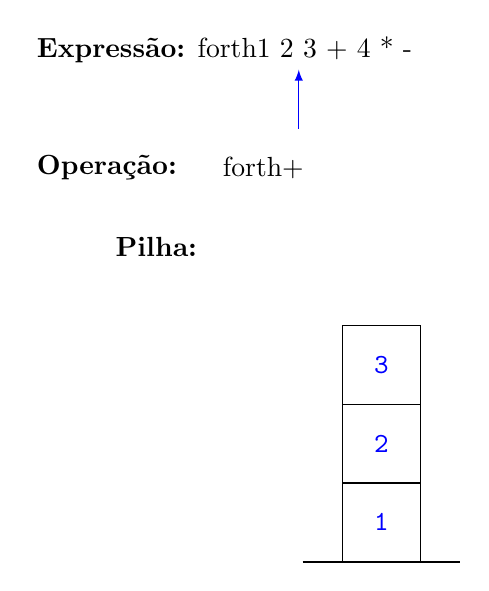
\begin{tikzpicture}
        \node[anchor=west] at (1, 6.5) { \textbf{Expressão:} \code{forth}{1 2 3 + 4 * -} };
        \node[anchor=west] at (1, 5) { \textbf{Operação:} };
        \node[anchor=west] at (2, 4) { \textbf{Pilha:} };
        
        \draw[thick] (4.5, 0) to (6.5, 0);

        \draw[-latex,color=blue] (4.45, 5.5) to (4.45, 6.25);

        \draw (5, 0) rectangle (6, 1);
        \node at (5.5, 0.5) { \tt \textcolor{blue}{1} };

        \draw (5, 1) rectangle (6, 2);
        \node at (5.5, 1.5) { \tt \textcolor{blue}{2} };

        \draw (5, 2) rectangle (6, 3);
        \node at (5.5, 2.5) { \tt \textcolor{blue}{3} };

        \pause

        \node at (4, 5) { \code{forth}{+} };

    \end{tikzpicture}

\end{frame}

\begin{frame}[fragile]{Exemplo de aritmética em Forth}

    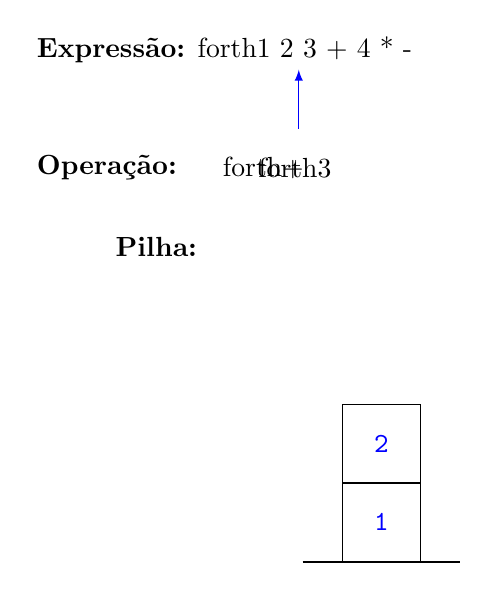
\begin{tikzpicture}
        \node[anchor=west] at (1, 6.5) { \textbf{Expressão:} \code{forth}{1 2 3 + 4 * -} };
        \node[anchor=west] at (1, 5) { \textbf{Operação:} };
        \node[anchor=west] at (2, 4) { \textbf{Pilha:} };
        
        \draw[thick] (4.5, 0) to (6.5, 0);

        \draw[-latex,color=blue] (4.45, 5.5) to (4.45, 6.25);

        \draw (5, 0) rectangle (6, 1);
        \node at (5.5, 0.5) { \tt \textcolor{blue}{1} };

        \draw (5, 1) rectangle (6, 2);
        \node at (5.5, 1.5) { \tt \textcolor{blue}{2} };

%        \draw (5, 2) rectangle (6, 3);
%        \node at (5.5, 2.5) { \tt \textcolor{blue}{3} };

        \node at (4, 5) { \code{forth}{+} };
        \node at (4.4, 5) { \code{forth}{3} };

    \end{tikzpicture}

\end{frame}

\begin{frame}[fragile]{Exemplo de aritmética em Forth}

    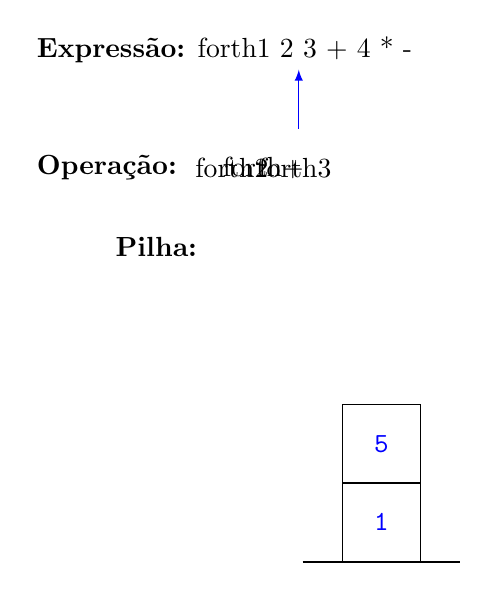
\begin{tikzpicture}
        \node[anchor=west] at (1, 6.5) { \textbf{Expressão:} \code{forth}{1 2 3 + 4 * -} };
        \node[anchor=west] at (1, 5) { \textbf{Operação:} };
        \node[anchor=west] at (2, 4) { \textbf{Pilha:} };
        
        \draw[thick] (4.5, 0) to (6.5, 0);

        \draw[-latex,color=blue] (4.45, 5.5) to (4.45, 6.25);

        \draw (5, 0) rectangle (6, 1);
        \node at (5.5, 0.5) { \tt \textcolor{blue}{1} };


%        \draw (5, 2) rectangle (6, 3);
%        \node at (5.5, 2.5) { \tt \textcolor{blue}{3} };

        \node at (4, 5) { \code{forth}{+} };
        \node at (4.4, 5) { \code{forth}{3} };
        \node at (3.6, 5) { \code{forth}{2} };

        \pause

        \draw (5, 1) rectangle (6, 2);
        \node at (5.5, 1.5) { \tt \textcolor{blue}{5} };

    \end{tikzpicture}

\end{frame}

\begin{frame}[fragile]{Exemplo de aritmética em Forth}

    \begin{tikzpicture}
        \node[anchor=west] at (1, 6.5) { \textbf{Expressão:} \code{forth}{1 2 3 + 4 * -} };
        \node[anchor=west] at (1, 5) { \textbf{Operação:} };
        \node[anchor=west] at (2, 4) { \textbf{Pilha:} };
        
        \draw[thick] (4.5, 0) to (6.5, 0);

        \draw[-latex,color=blue] (4.85, 5.5) to (4.85, 6.25);

        \draw (5, 0) rectangle (6, 1);
        \node at (5.5, 0.5) { \tt \textcolor{blue}{1} };

        \draw (5, 1) rectangle (6, 2);
        \node at (5.5, 1.5) { \tt \textcolor{blue}{5} };

        \pause

        \draw (5, 2) rectangle (6, 3);
        \node at (5.5, 2.5) { \tt \textcolor{blue}{4} };

%        \node at (4, 5) { \code{forth}{+} };
%        \node at (4.4, 5) { \code{forth}{3} };
%        \node at (3.6, 5) { \code{forth}{2} };

    \end{tikzpicture}

\end{frame}

\begin{frame}[fragile]{Exemplo de aritmética em Forth}

    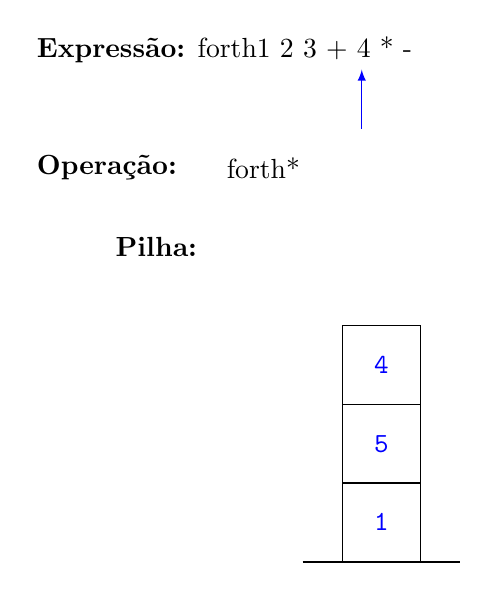
\begin{tikzpicture}
        \node[anchor=west] at (1, 6.5) { \textbf{Expressão:} \code{forth}{1 2 3 + 4 * -} };
        \node[anchor=west] at (1, 5) { \textbf{Operação:} };
        \node[anchor=west] at (2, 4) { \textbf{Pilha:} };
        
        \draw[thick] (4.5, 0) to (6.5, 0);

        \draw[-latex,color=blue] (5.25, 5.5) to (5.25, 6.25);

        \draw (5, 0) rectangle (6, 1);
        \node at (5.5, 0.5) { \tt \textcolor{blue}{1} };

        \draw (5, 1) rectangle (6, 2);
        \node at (5.5, 1.5) { \tt \textcolor{blue}{5} };

        \draw (5, 2) rectangle (6, 3);
        \node at (5.5, 2.5) { \tt \textcolor{blue}{4} };

        \pause
        \node at (4, 5) { \code{forth}{*} };
%        \node at (4.4, 5) { \code{forth}{3} };
%        \node at (3.6, 5) { \code{forth}{2} };

    \end{tikzpicture}

\end{frame}

\begin{frame}[fragile]{Exemplo de aritmética em Forth}

    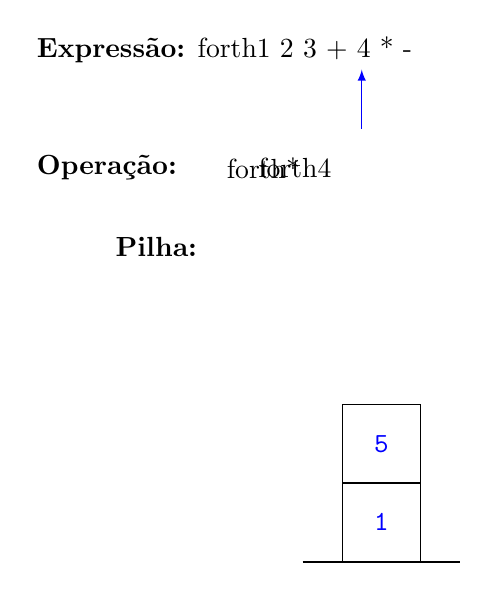
\begin{tikzpicture}
        \node[anchor=west] at (1, 6.5) { \textbf{Expressão:} \code{forth}{1 2 3 + 4 * -} };
        \node[anchor=west] at (1, 5) { \textbf{Operação:} };
        \node[anchor=west] at (2, 4) { \textbf{Pilha:} };
        
        \draw[thick] (4.5, 0) to (6.5, 0);

        \draw[-latex,color=blue] (5.25, 5.5) to (5.25, 6.25);

        \draw (5, 0) rectangle (6, 1);
        \node at (5.5, 0.5) { \tt \textcolor{blue}{1} };

        \draw (5, 1) rectangle (6, 2);
        \node at (5.5, 1.5) { \tt \textcolor{blue}{5} };

%        \draw (5, 2) rectangle (6, 3);
%        \node at (5.5, 2.5) { \tt \textcolor{blue}{4} };

        \node at (4, 5) { \code{forth}{*} };
        \node at (4.4, 5) { \code{forth}{4} };
%        \node at (3.6, 5) { \code{forth}{2} };

    \end{tikzpicture}

\end{frame}

\begin{frame}[fragile]{Exemplo de aritmética em Forth}

    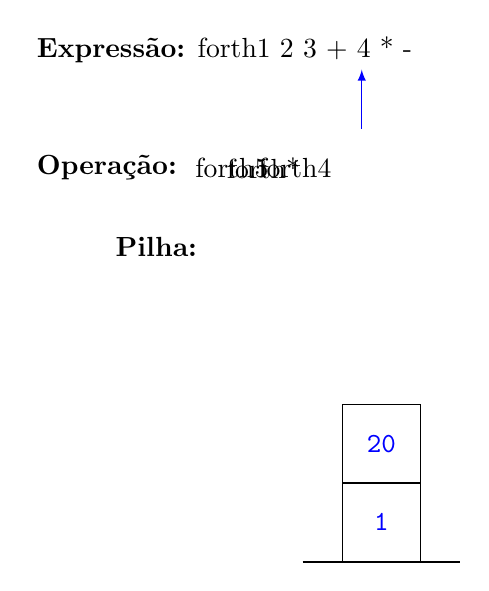
\begin{tikzpicture}
        \node[anchor=west] at (1, 6.5) { \textbf{Expressão:} \code{forth}{1 2 3 + 4 * -} };
        \node[anchor=west] at (1, 5) { \textbf{Operação:} };
        \node[anchor=west] at (2, 4) { \textbf{Pilha:} };
        
        \draw[thick] (4.5, 0) to (6.5, 0);

        \draw[-latex,color=blue] (5.25, 5.5) to (5.25, 6.25);

        \draw (5, 0) rectangle (6, 1);
        \node at (5.5, 0.5) { \tt \textcolor{blue}{1} };

        \node at (4, 5) { \code{forth}{*} };
        \node at (4.4, 5) { \code{forth}{4} };
        \node at (3.6, 5) { \code{forth}{5} };

        \pause

        \draw (5, 1) rectangle (6, 2);
        \node at (5.5, 1.5) { \tt \textcolor{blue}{20} };

    \end{tikzpicture}

\end{frame}

\begin{frame}[fragile]{Exemplo de aritmética em Forth}

    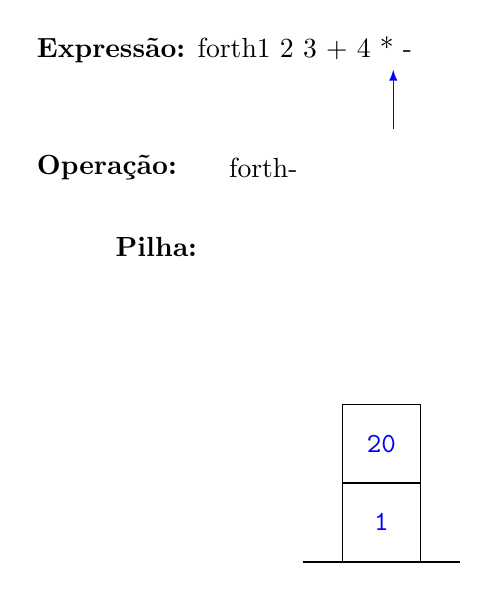
\begin{tikzpicture}
        \node[anchor=west] at (1, 6.5) { \textbf{Expressão:} \code{forth}{1 2 3 + 4 * -} };
        \node[anchor=west] at (1, 5) { \textbf{Operação:} };
        \node[anchor=west] at (2, 4) { \textbf{Pilha:} };
        
        \draw[thick] (4.5, 0) to (6.5, 0);

        \draw[-latex,color=blue] (5.65, 5.5) to (5.65, 6.25);

        \draw (5, 0) rectangle (6, 1);
        \node at (5.5, 0.5) { \tt \textcolor{blue}{1} };

        \draw (5, 1) rectangle (6, 2);
        \node at (5.5, 1.5) { \tt \textcolor{blue}{20} };

        \pause

        \node at (4, 5) { \code{forth}{-} };
        %\node at (4.4, 5) { \code{forth}{4} };
        %\node at (3.6, 5) { \code{forth}{5} };

    \end{tikzpicture}

\end{frame}

\begin{frame}[fragile]{Exemplo de aritmética em Forth}

    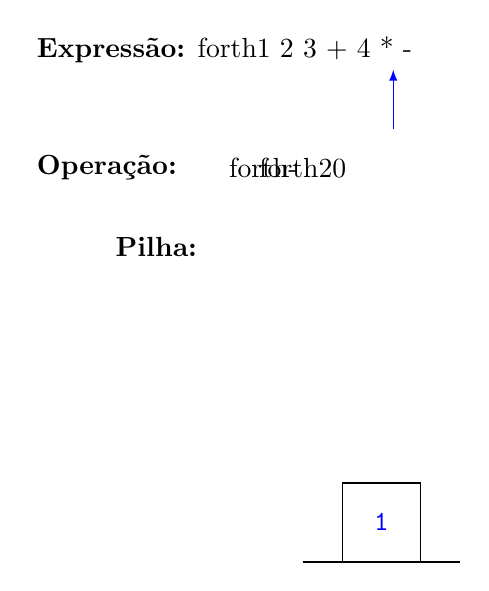
\begin{tikzpicture}
        \node[anchor=west] at (1, 6.5) { \textbf{Expressão:} \code{forth}{1 2 3 + 4 * -} };
        \node[anchor=west] at (1, 5) { \textbf{Operação:} };
        \node[anchor=west] at (2, 4) { \textbf{Pilha:} };
        
        \draw[thick] (4.5, 0) to (6.5, 0);

        \draw[-latex,color=blue] (5.65, 5.5) to (5.65, 6.25);

        \draw (5, 0) rectangle (6, 1);
        \node at (5.5, 0.5) { \tt \textcolor{blue}{1} };

        \node at (4, 5) { \code{forth}{-} };
        \node at (4.5, 5) { \code{forth}{20} };
        %\node at (3.6, 5) { \code{forth}{5} };

    \end{tikzpicture}

\end{frame}

\begin{frame}[fragile]{Exemplo de aritmética em Forth}

    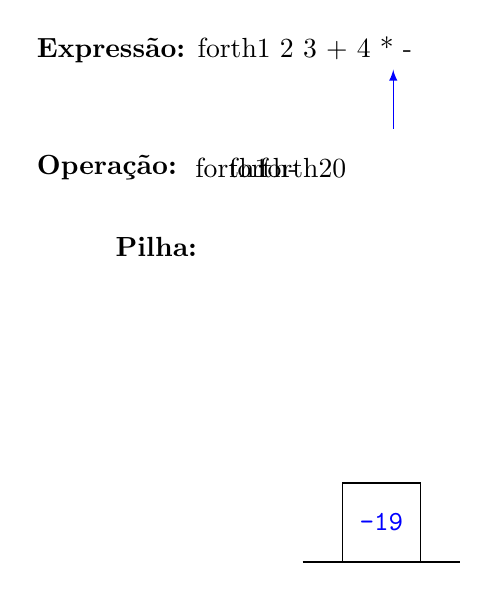
\begin{tikzpicture}
        \node[anchor=west] at (1, 6.5) { \textbf{Expressão:} \code{forth}{1 2 3 + 4 * -} };
        \node[anchor=west] at (1, 5) { \textbf{Operação:} };
        \node[anchor=west] at (2, 4) { \textbf{Pilha:} };
        
        \draw[thick] (4.5, 0) to (6.5, 0);

        \draw[-latex,color=blue] (5.65, 5.5) to (5.65, 6.25);

        \node at (4, 5) { \code{forth}{-} };
        \node at (4.5, 5) { \code{forth}{20} };
        \node at (3.6, 5) { \code{forth}{1} };

        \pause

        \draw (5, 0) rectangle (6, 1);
        \node at (5.5, 0.5) { \tt \textcolor{blue}{-19} };
    \end{tikzpicture}

\end{frame}



\begin{frame}[fragile]{Notação posfixa}

    \begin{itemize}
        \item Forth utiliza de notação posfixa, isto, as palavras sucedem seus operandos, conforme
            ilustrado no exemplo anterior

        \item Esta convenção permite que a pilha seja preparada antes da execução de uma palavra e que
            as palavras extraiam seus argumentos, quando existirem, da pilha, em ordem reversa: do
            último para o primeiro argumento

        \item O código abaixo corresponde ao exemplo anterior: a palavra \code{forth}{.} (ponto final)
            extrai o topo da pilha e o imprime no terminal

            \inputcode{forth}{codes/expr.fs}

            \vspace{0.1in}
        
        \item Observe que, ao final da execução, a pilha estará vazia

    \end{itemize}

\end{frame}

\begin{frame}[fragile]{\textit{Stack underflow, stack overflow} e \textit{stack effects}}

    \begin{itemize}
        \item A tentativa de se extrair um elemento quando a pilha está vazia resulta no erro
            \textit{stack underflow}:

            \inputcode{forth}{codes/underflow.fs}
            \vspace{0.1in}

        \item Se não houver memória disponível para a inserção de um novo elemento na pilha, o 
            interpretador emitirá o erro \textit{stack overflow}

        \item Tanto as palavras já definidas por Forth quanto as palavras definidas pelo usuário
            podem tanto extrair elementos da pilha quanto inserir novos elementos

        \item Estas inserções ou remoções são denominadas \textit{stack effects}

        \item Estes efeitos podem ser registrados por meio de um comentário que é inserido, na 
            definição de uma nova palavra, entre o nome e a implementação
    \end{itemize}

\end{frame}

\begin{frame}[fragile]{Notação de pilha}

    \begin{itemize}
        \item O comentário que registra os  \textit{stack effects} da palavra é denominado
            \textbf{notação de pilha}

        \item A forma básica da notação de pilha é

            \inputsyntax{forth}{codes/notation.fs}

        onde \textit{before} registra o que deve estar na \textit{stack} antes da execução e
        \textit{after} regista o que estará na \textit{stack} após a execução

        \item A notação de pilha para a palavra \code{forth}{.} é 

            \inputsyntax{forth}{codes/dot.fs}

        \item A notação de pilha para a palavra \code{forth}{+} é 

            \inputsyntax{forth}{codes/sum.fs}

    \end{itemize}

\end{frame}

\begin{frame}[fragile]{Sumário}

    \begin{scriptsize}
    \begin{table}
        \centering
        \begin{tabularx}{0.95\textwidth}{ccX}
            \toprule
            \textbf{Palavra} & \textbf{Notação de pilha} & \textbf{Significado} \\
            \midrule
            \code{forth}{: name impl ;} & \code{forth}{( -- )} & Define a palavra \code{forth}{name} por meio das palavras \code{forth}{impl} \\
            \midrule
            \code{forth}{CR} & \code{forth}{( -- )} & Imprime uma nova linha \\
            \midrule
            \code{forth}{SPACES} & \code{forth}{( n -- )} & Imprime $n$ espaços \\
            \midrule
            \code{forth}{EMIT} & \code{forth}{( c -- )} & Imprime o caractere $c$ \\
            \midrule
            \code{forth}{."} & \code{forth}{( -- )} & Imprime a string delimitada por \code{forth}{"} que se segue\\
            \midrule
            \code{forth}{.} & \code{forth}{( n -- )} & Imprime o número $n$, seguido de um espaço $c$ \\
            \midrule
            \code{forth}{+} & \code{forth}{( n1 n2 -- s )} & Computa $s = n1 + n2$ \\
            \midrule
            \code{forth}{-} & \code{forth}{( n1 n2 -- s )} & Computa $s = n1 - n2$ \\
            \midrule
            \code{forth}{*} & \code{forth}{( n1 n2 -- m )} & Computa $m = n1 \times n2$ \\
            \midrule
            \code{forth}{/} & \code{forth}{( n1 n2 -- q )} & Computa o quociente $q$ da divisão inteira de $n1$ por $n2$ \\
            \midrule
            \code{forth}{MOD} & \code{forth}{( n1 n2 -- r )} & Computa o resto $r$ da divisão inteira de $n1$ por $n2$ \\
            \midrule
            \code{forth}{/MOD} & \code{forth}{( n1 n2 -- q r )} & Computa o quociente $q$ e o resto $r$ da divisão de $n1$ por $n2$ \\
            \bottomrule
        \end{tabularx}
    \end{table}
    \end{scriptsize}

\end{frame}

\begin{frame}[fragile]{Exemplo: conversão de tempo}
    \inputcode{forth}{codes/time.fs}
\end{frame}

\begin{frame}[fragile]{Exemplo: movimento retilíneo uniforme}
    \inputcode{forth}{codes/mu.fs}
\end{frame}
